\section{Gestures}
In this section the gestures are described.
The effect of each gesture is described in Jerome\rq{}s documentation.

\subsection{Fire}
The fire gesture (see~\autoref{fig:fire-gesture}) is a flame symbol drawn from left to right.
It is defined by this trajectory:

\begin{lstlisting}
Trajectory{
    {0,  0, 0},
    {-1, 3, 0},
    {1,  2, 0},
    {2,  5, 0},
    {2,  5, 0},
    {3,  2, 0},
    {5,  3, 0},
    {4,  0, 0},
}
\end{lstlisting}

\begin{figure}[!ht]
    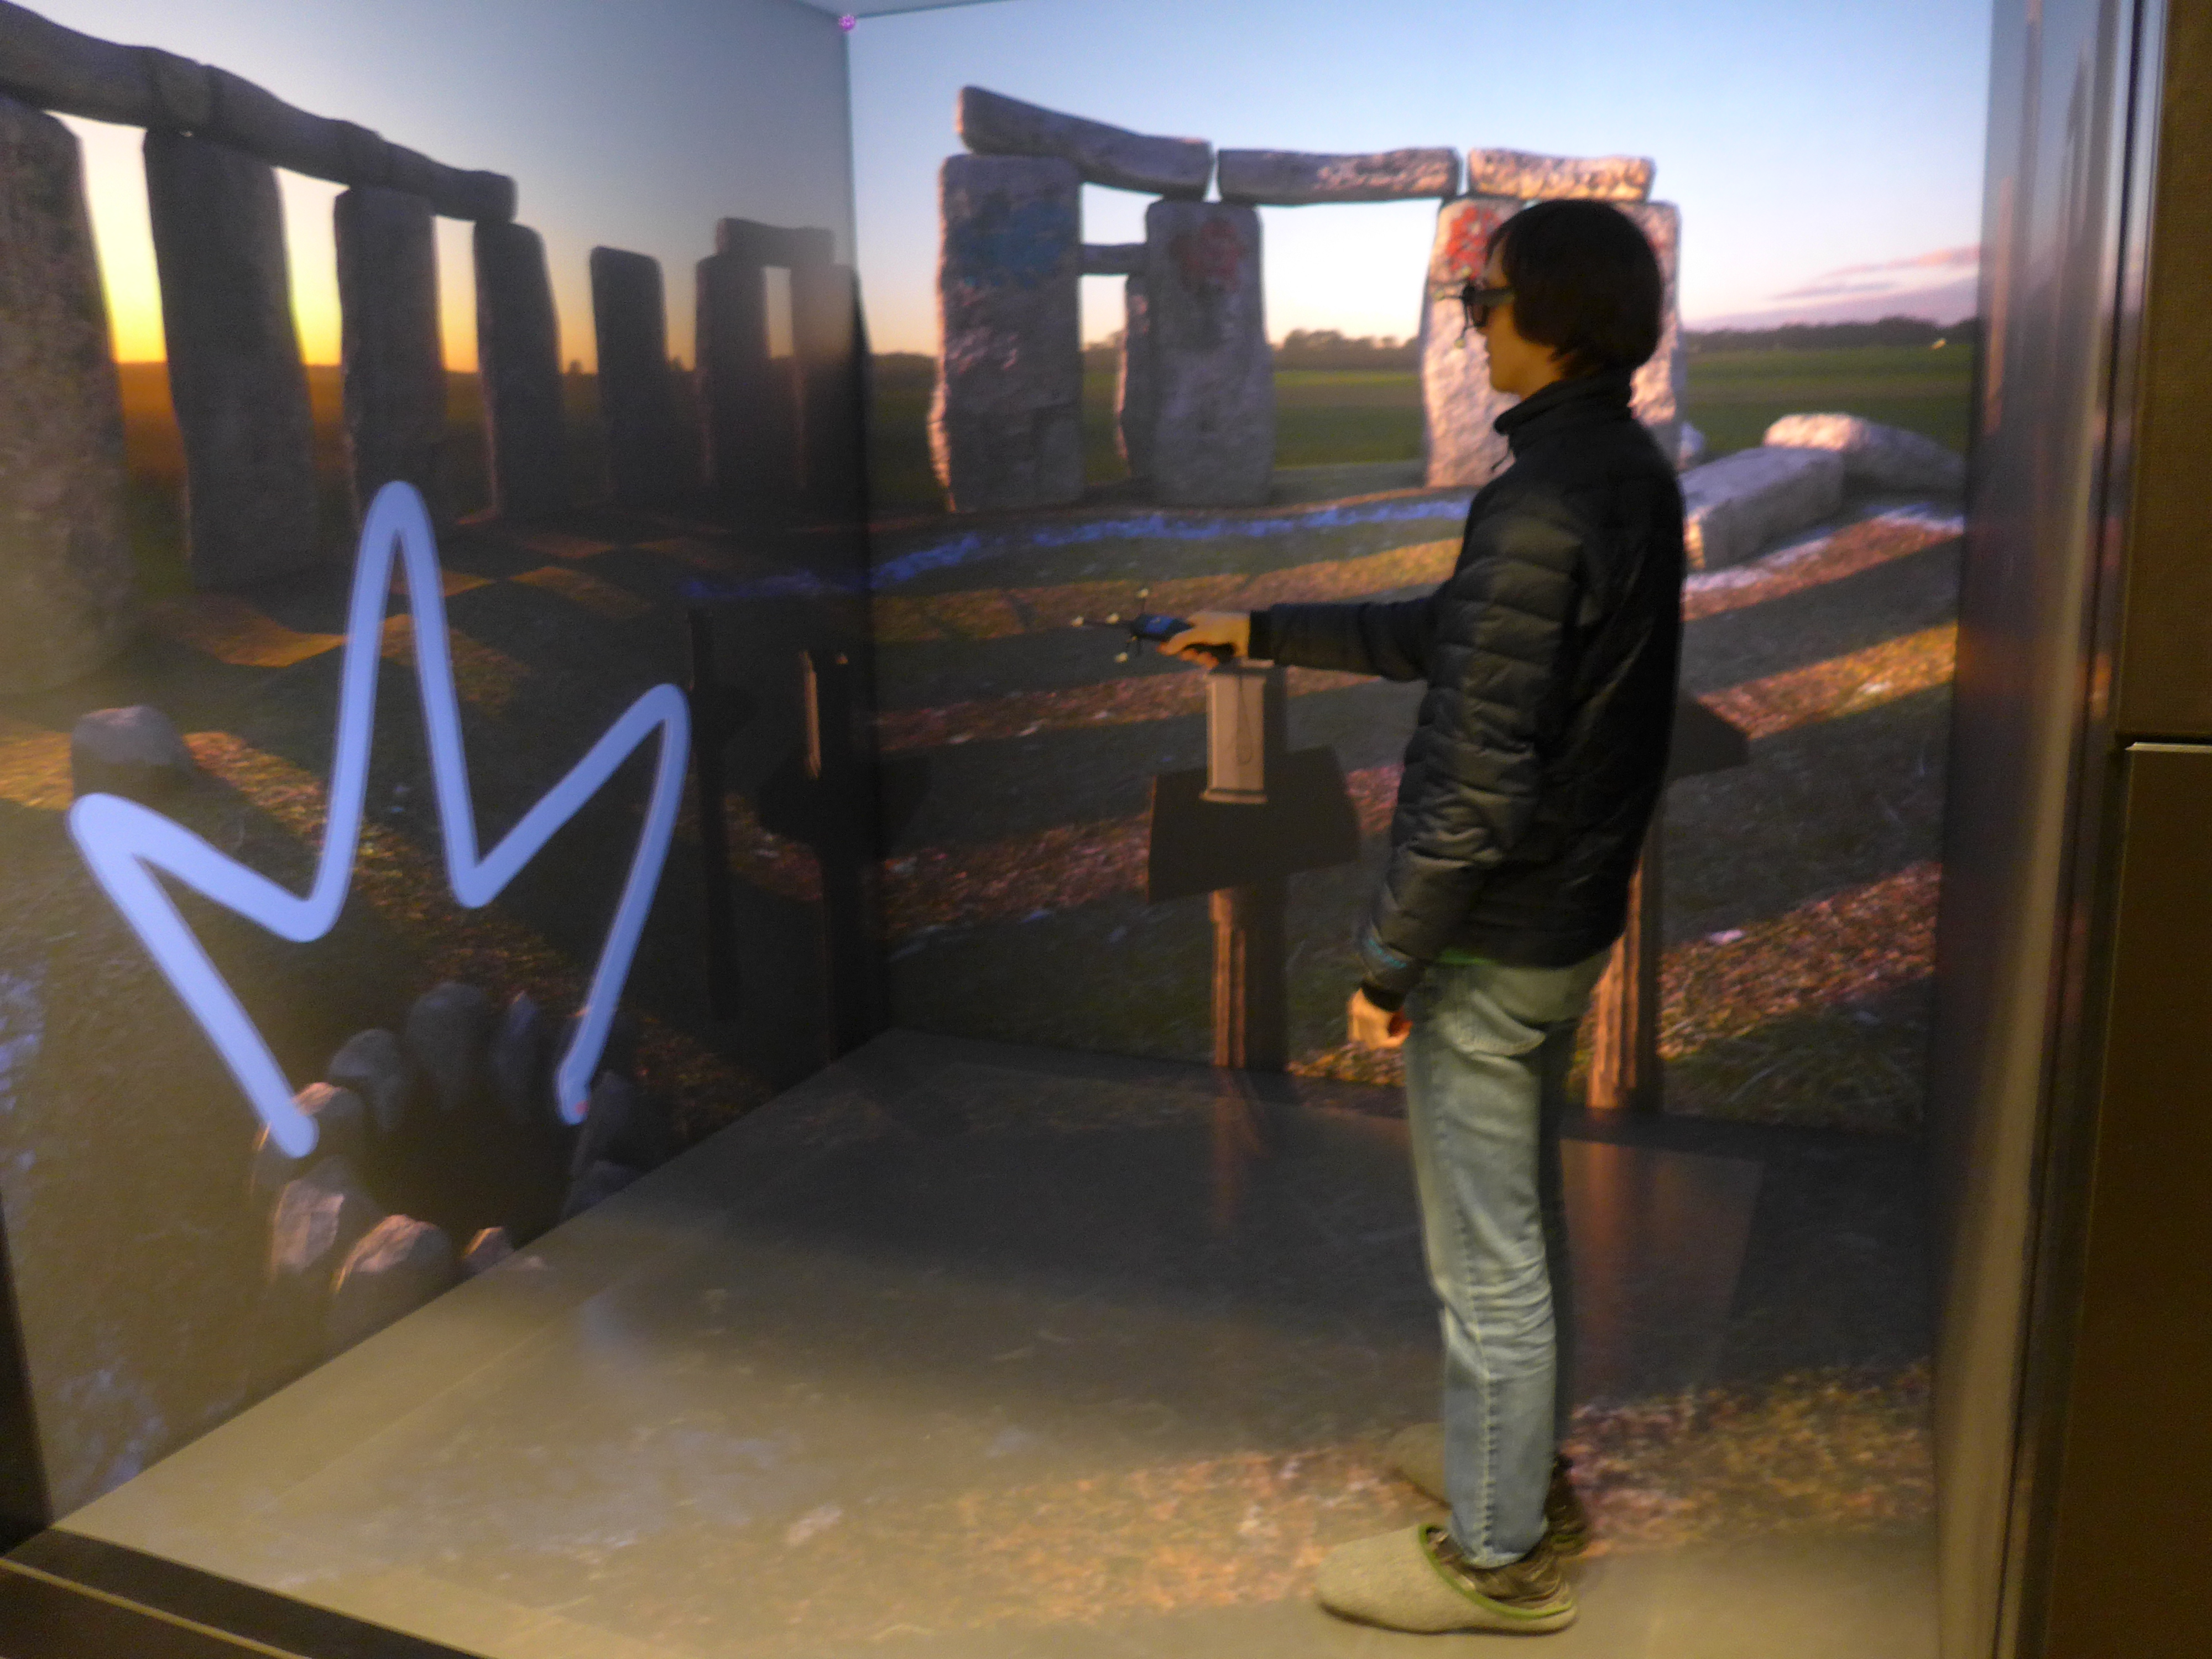
\includegraphics[width=0.4\textwidth]{pictures/fire-gesture.jpg}
    \caption{Fire gesture}
    \label{fig:fire-gesture}
\end{figure}


\subsection{Water}
The water gesture (see~\autoref{fig:water-gesture}) is a wave symbol drawn from left to right.
It is defined by this bezier curve:

\begin{lstlisting}
const BezierCurve<> waterBezier{
    {0,    0,  0},
    {1.5f, 3,  0},
    {1.5f, -2, 0},
    {3,    1,  0},
};
\end{lstlisting}

\begin{figure}[!ht]
    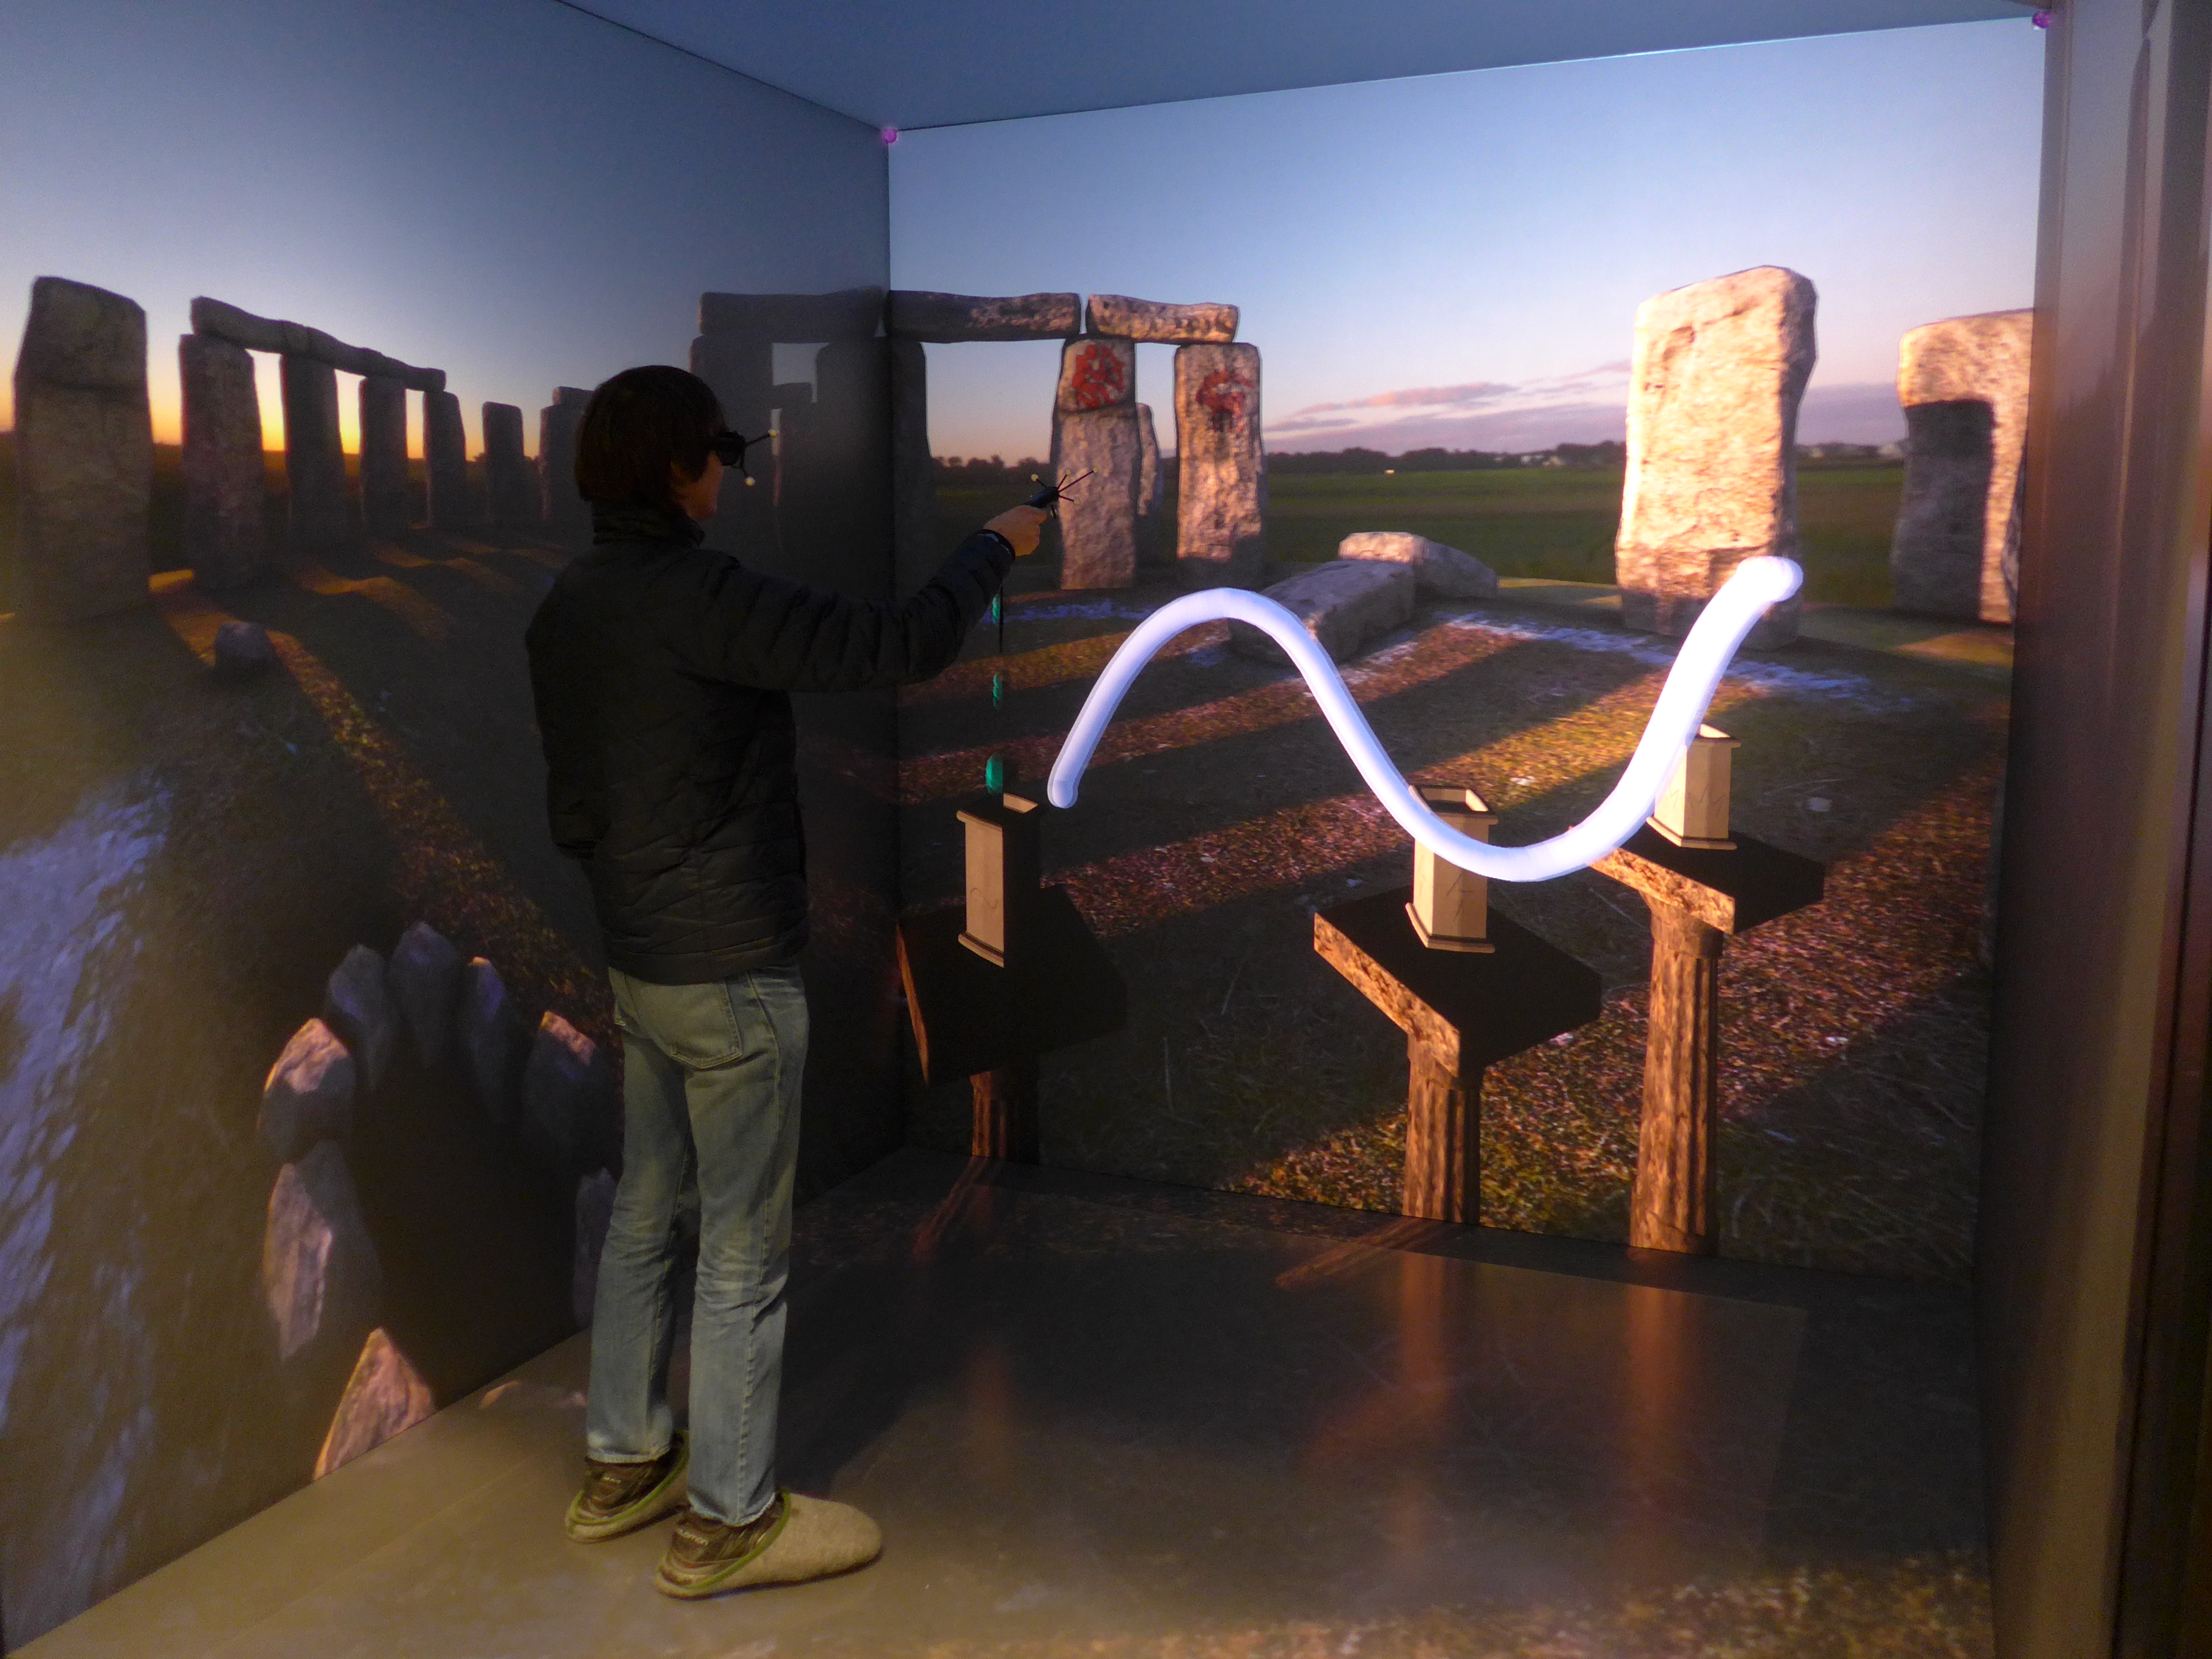
\includegraphics[width=0.4\textwidth]{pictures/water-gesture.jpg}
    \caption{Water gesture}
    \label{fig:water-gesture}
\end{figure}


\subsection{Lightning}
The lightning gesture (see~\autoref{fig:lightning-gesture}) is a lightning symbol drawn from top to bottom.
It is defined by this trajectory:

\begin{lstlisting}
Trajectory{
    {1, 2, 0},
    {0, 1, 0},
    {1, 1, 0},
    {0, 0, 0},
}
\end{lstlisting}

\begin{figure}[!ht]
    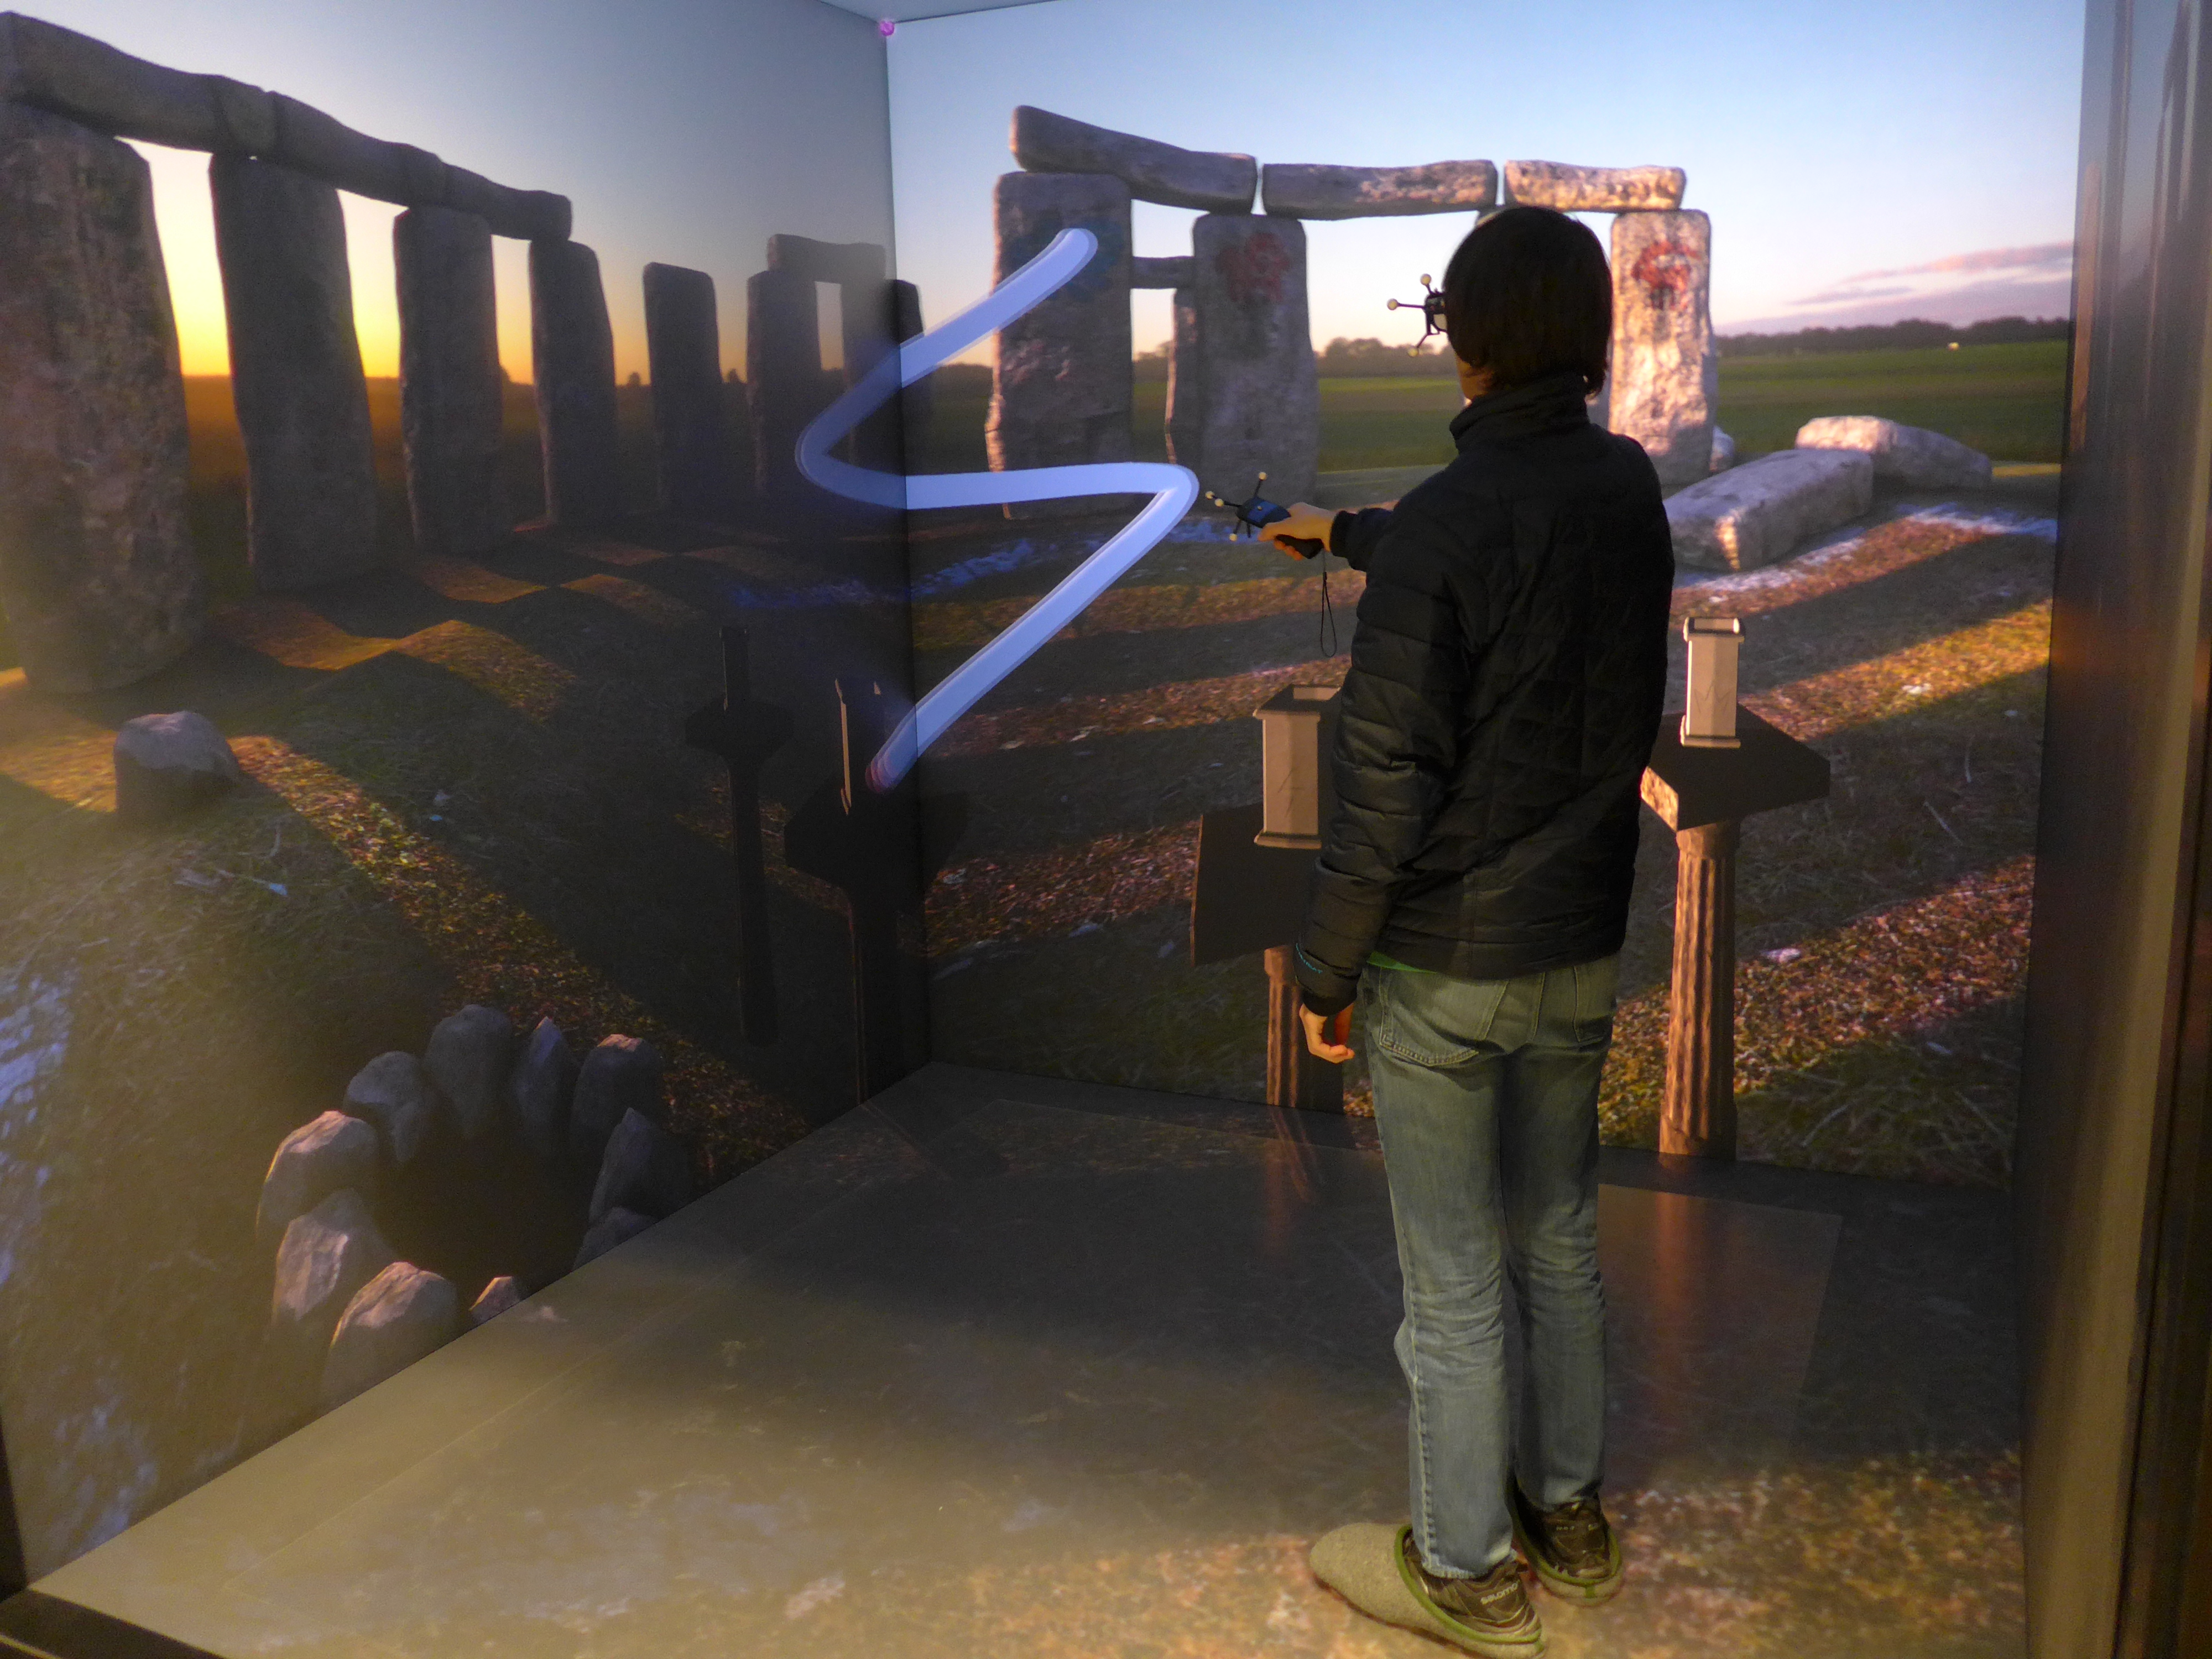
\includegraphics[width=0.4\textwidth]{pictures/lightning-gesture.jpg}
    \caption{Lightning gesture}
    \label{fig:lightning-gesture}
\end{figure}


\subsection{Wind}
The wind gesture (see~\autoref{fig:wind-gesture}) is a spiral drawn from the inside to the outside.
The trajectory is calculated in the method \inlineCpp{sample} of the class \path{sources/magicvr/Spiral.cpp}.

\begin{figure}[!ht]
    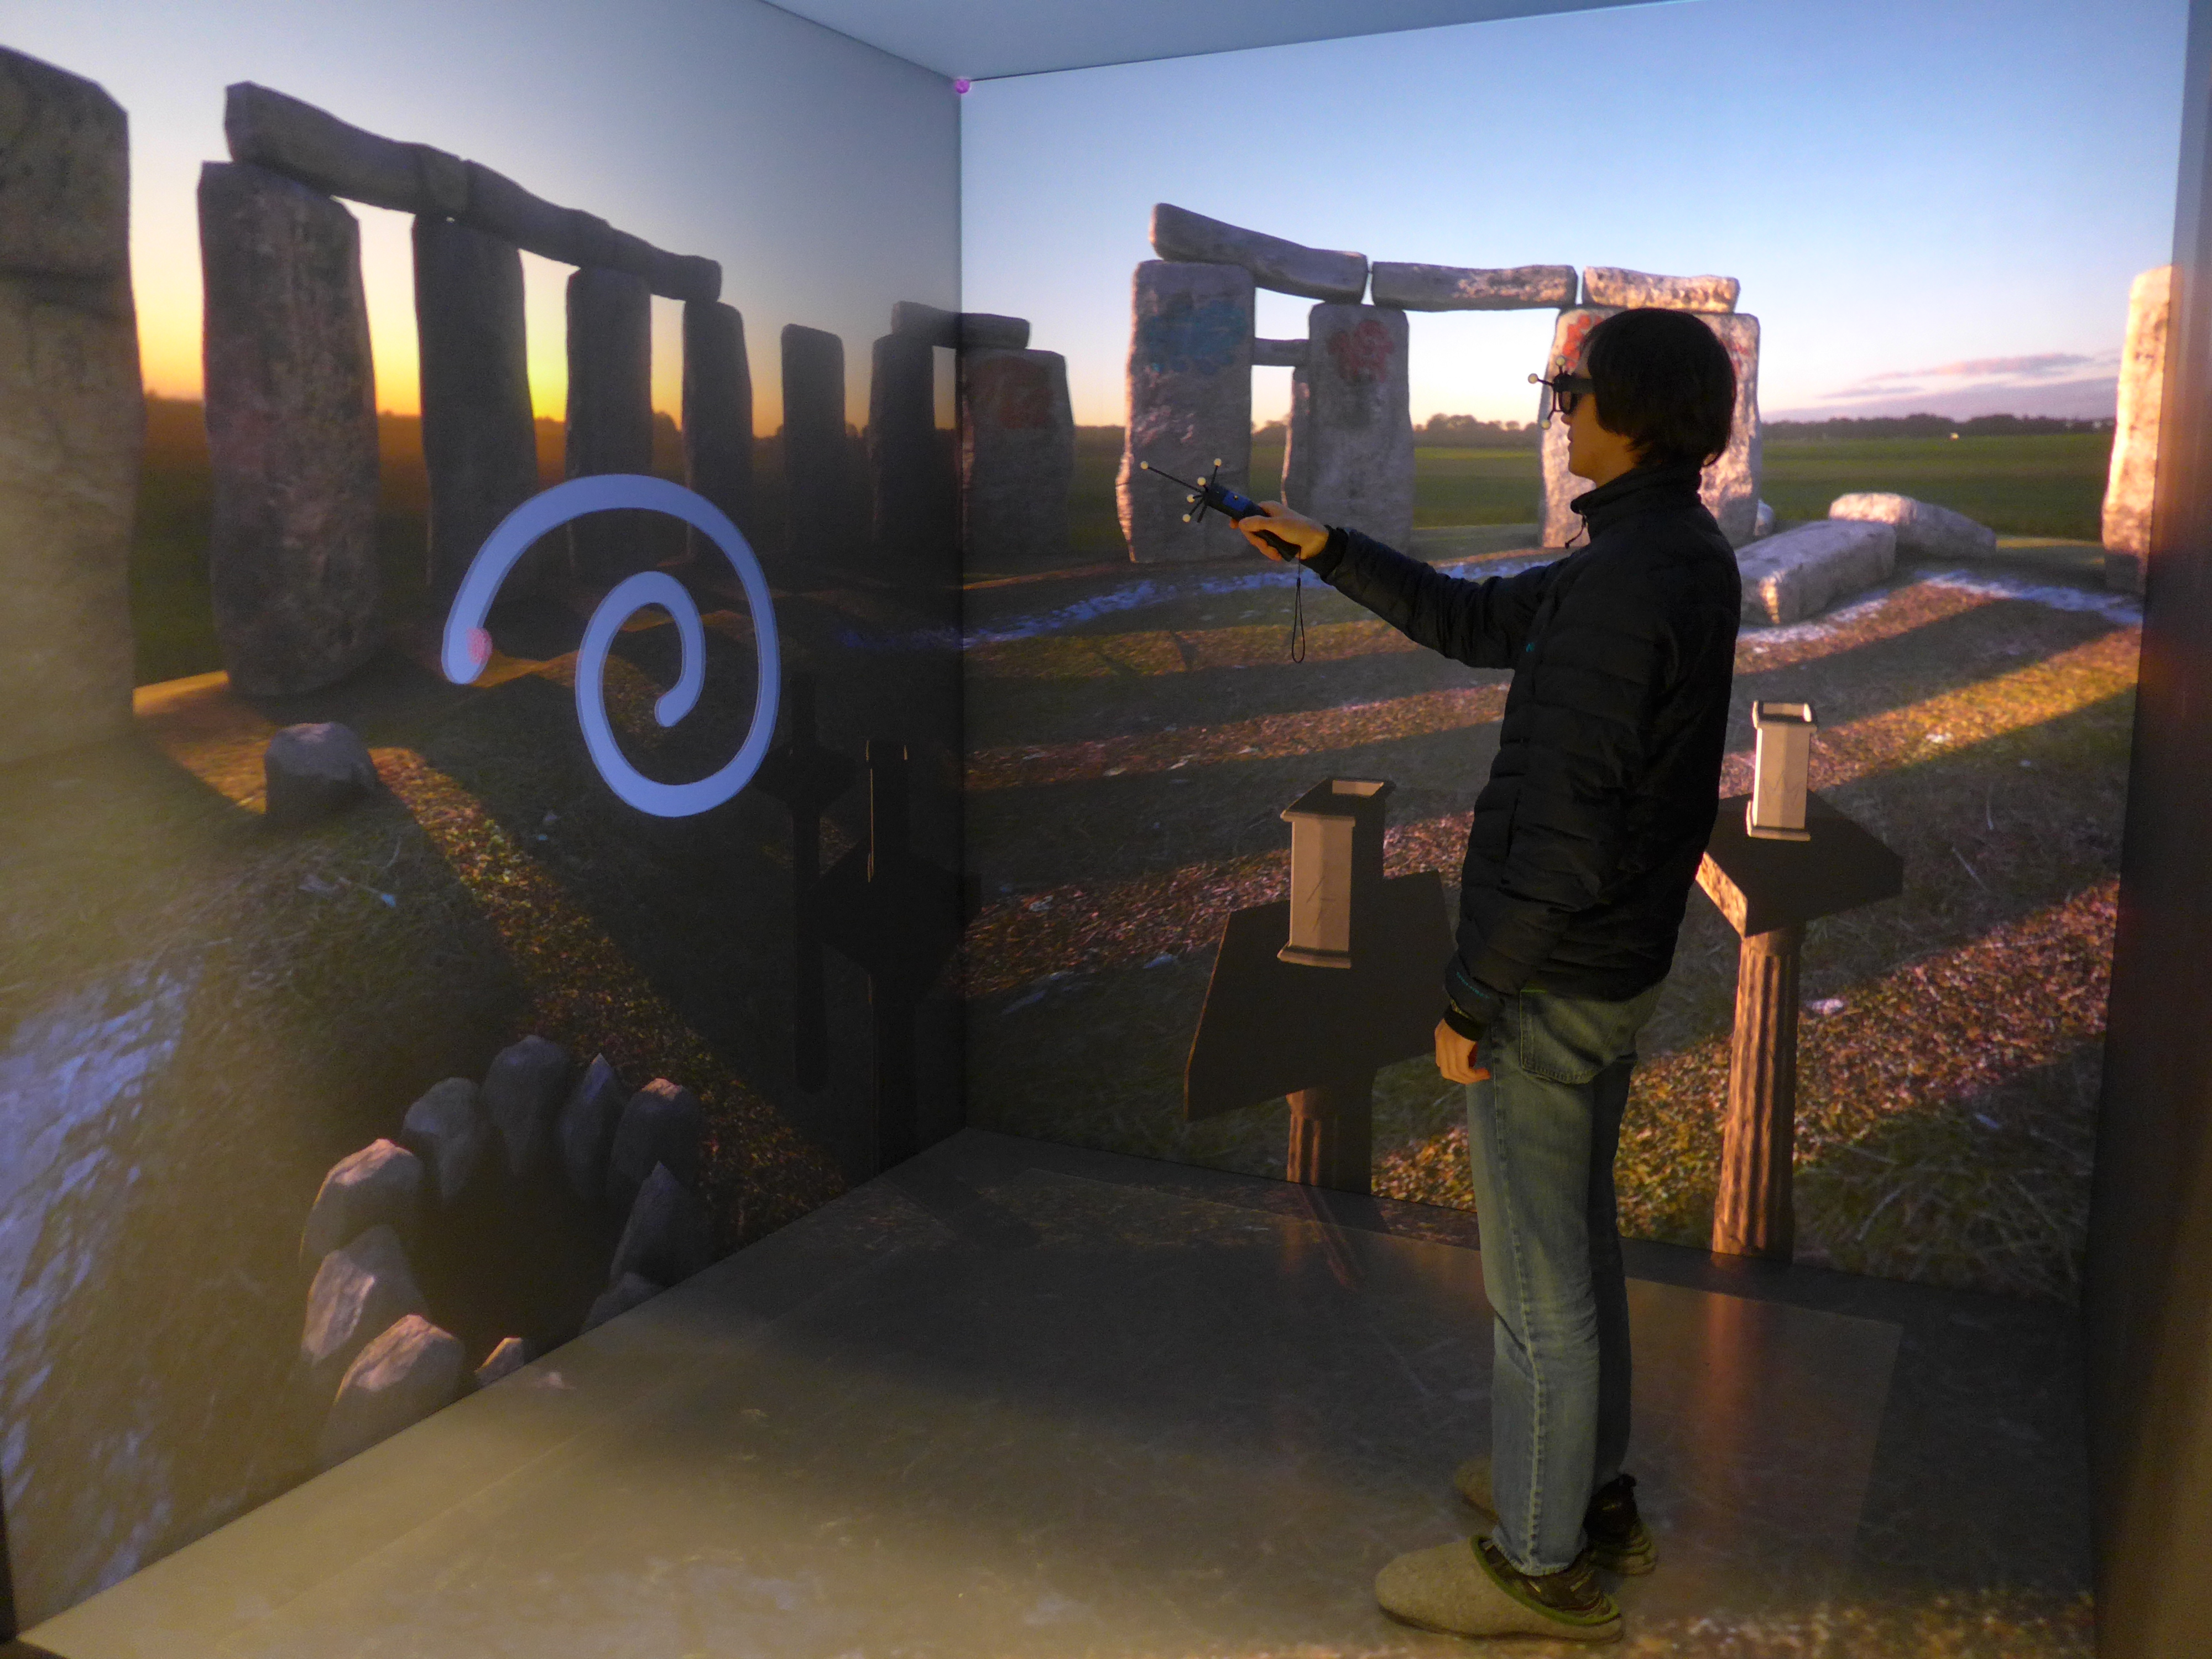
\includegraphics[width=0.4\textwidth]{pictures/wind-gesture.jpg}
    \caption{Wind gesture}
    \label{fig:wind-gesture}
\end{figure}


\subsection{Circle}\label{subsec:circle}
The circle gesture (see~\autoref{fig:circle-gesture}) is a single circle drawn from the left side of the center to the top.
The trajectory is calculated in the method \inlineCpp{sample} of the class \path{sources/magicvr/ranges/view/Circle.cpp}.

\begin{lstlisting}
Circle(1).sample(0, 360, 10)
\end{lstlisting}

\begin{figure}[!ht]
    \centering
    \includegraphics[width=0.15\textwidth]{pictures/circle-gesture.png}
    \caption{Circle gesture}
    \label{fig:circle-gesture}
\end{figure}


\subsection{Multiplication}
The multiplication gesture is a~\nameref{subsec:circle} gesture with two circumnavigations.

\begin{lstlisting}
Circle(1).sample(0, 720, 10)
\end{lstlisting}


\subsection{Shoot}
The shoot gesture (see~\autoref{fig:shoot-gesture}) is a quarter segment of a circle drawn from above with a circumnavigation direction to the right (in the style of a whip movement).

\begin{lstlisting}
const BezierCurve<> quaterCircleFromAbove{
        {0, 1, 0},
        {1, 1, 0},
        {1, 0, 0},
        {1, 0, 0},
};
\end{lstlisting}

\begin{figure}[!ht]
    \centering
    \includegraphics[width=0.15\textwidth]{pictures/shoot-gesture.png}
    \caption{Shoot gesture}
    \label{fig:shoot-gesture}
\end{figure}